\documentclass{sigchi}

% Use this command to override the default ACM copyright statement
% (e.g. for preprints).  Consult the conference website for the
% camera-ready copyright statement.

%% EXAMPLE BEGIN -- HOW TO OVERRIDE THE DEFAULT COPYRIGHT STRIP -- (July 22, 2013 - Paul Baumann)
% \toappear{Permission to make digital or hard copies of all or part of this work for personal or classroom use is      granted without fee provided that copies are not made or distributed for profit or commercial advantage and that copies bear this notice and the full citation on the first page. Copyrights for components of this work owned by others than ACM must be honored. Abstracting with credit is permitted. To copy otherwise, or republish, to post on servers or to redistribute to lists, requires prior specific permission and/or a fee. Request permissions from permissions@acm.org. \\
% {\emph{CHI'14}}, April 26--May 1, 2014, Toronto, Canada. \\
% Copyright \copyright~2014 ACM ISBN/14/04...\$15.00. \\
% DOI string from ACM form confirmation}
%% EXAMPLE END -- HOW TO OVERRIDE THE DEFAULT COPYRIGHT STRIP -- (July 22, 2013 - Paul Baumann)

% Arabic page numbers for submission.  Remove this line to eliminate
% page numbers for the camera ready copy 
% \pagenumbering{arabic}

% Load basic packages
\usepackage{balance}  % to better equalize the last page
\usepackage{graphics} % for EPS, load graphicx instead 
%\usepackage[T1]{fontenc}
\usepackage{txfonts}
\usepackage{times}    % comment if you want LaTeX's default font
\usepackage[pdftex]{hyperref}
% \usepackage{url}      % llt: nicely formatted URLs
\usepackage{color}
\usepackage{textcomp}
\usepackage{booktabs}
\usepackage{ccicons}
\usepackage{todonotes}

\usepackage[font=normalsize,labelfont=bf]{caption}
\usepackage{subcaption}

\usepackage[acronym]{glossaries}

% llt: Define a global style for URLs, rather that the default one
\makeatletter
\def\url@leostyle{%
  \@ifundefined{selectfont}{\def\UrlFont{\sf}}{\def\UrlFont{\small\bf\ttfamily}}}
\makeatother
\urlstyle{leo}

% To make various LaTeX processors do the right thing with page size.
\def\pprw{8.5in}
\def\pprh{11in}
\special{papersize=\pprw,\pprh}
\setlength{\paperwidth}{\pprw}
\setlength{\paperheight}{\pprh}
\setlength{\pdfpagewidth}{\pprw}
\setlength{\pdfpageheight}{\pprh}

% Make sure hyperref comes last of your loaded packages, to give it a
% fighting chance of not being over-written, since its job is to
% redefine many LaTeX commands.
\definecolor{linkColor}{RGB}{6,125,233}
\hypersetup{%
  pdftitle={SIGCHI Conference Proceedings Format},
  pdfauthor={LaTeX},
  pdfkeywords={SIGCHI, proceedings, archival format},
  bookmarksnumbered,
  pdfstartview={FitH},
  colorlinks,
  citecolor=black,
  filecolor=black,
  linkcolor=black,
  urlcolor=linkColor,
  breaklinks=true,
}

% create a shortcut to typeset table headings
% \newcommand\tabhead[1]{\small\textbf{#1}}


% End of preamble. Here it comes the document.
\begin{document}

\title{From Large Touch Walls to Tablets -- a Responsive Web Framework for Large Multi-Touch Wall Applications}

\numberofauthors{3}
\author{%
  \alignauthor{1st Author Name\\
    \affaddr{Affiliation}\\
    \affaddr{City, Country}\\
    \email{e-mail address}}\\
  \alignauthor{2nd Author Name\\
    \affaddr{Affiliation}\\
    \affaddr{City, Country}\\
    \email{e-mail address}}\\
  \alignauthor{3rd Author Name\\
    \affaddr{Affiliation}\\
    \affaddr{City, Country}\\
    \email{e-mail address}}\\
}

\maketitle

\newacronym{spa}{SPA}{single-page application}
\newacronym{dom}{DOM}{Document Object Mode}
\newacronym{rwd}{RWD}{responsive web design}
\newacronym{sp2}{SP2}{second sprint planning}



\begin{abstract}
We present Awall, a responsive web application framework that supports collaborative teamwork using tablets and a large multi-touch wall system. 
The application was initially developed for large multi-touch walls. 
Further development revealed the need to interact with the system using a tablet. 
This presents unique challenges in respect to the UI and the flow of information. 
We describe Awall's architecture and implementation followed by the implemented application for the second sprint planning meeting in the agile software development process to showcase the responsive and collaborative nature of the application.
\end{abstract}

\category{H.5.2.}{Information Interfaces and Presentation (e.g. HCI)}{User Interfaces -- \textit{Interaction styles}}
\category{H.5.3.}{Information Interfaces and Presentation (e.g. HCI)}{Group and Organization Interfaces -- \textit{Computer-supported cooperative work}}
\category{H.5.4.}{Information Interfaces and Presentation (e.g. HCI)}{Hypertext/Hypermedia -- \textit{Architectures}}


\keywords{Responsive design; agile; second sprint planning; collaborative work; multi-touch; wall; tablets; web components}

\section{Introduction}
% agile sw dev intro
Agile promises that a project is finished on time, delivers high quality software, well constructed and maintainable code and that agile teams make the users happy \cite{Stellman:2014}.
The core of agile is a set of practices and methodologies around self-organizing teams relying on face-to-face communication \cite{Cockburn:2001}.
According to recent study in Switzerland, 70\% of all IT companies practice agile software development and 83\% of all IT professionals \cite{Kropp:2015}.
Agile software development projects are split into short iterations usually lasting between 2-4 weeks.
These iterations are called sprints.
% What is SP2?
The work that needs to be done is described in user stories, a short description of a feature in everyday language.
User stories are kept in the product backlog and are owned by the product owner.
At the beginning of a sprint, a set of user stories is selected for the iteration.
In a meeting called \gls{sp2}, the team then splits these user stories into smaller technical tasks that should not take longer than one workday to complete.
The traditional way to this is to write paper-notes and attach them to a wall.
The setup on the wall is called the taskboard and shows the progress of the team during the sprint.

% paper to digital
Replacing this paper-based solution with a digital, multi-touch wall requires the application to behave very similar to the paper-based wall. 
With the same possibilities and interactions.
% - tablets for collaborative work
The agile software development process has different meetings. 
For some the multi-touch wall alone is enough, for others more input sources are required. 
For that purpose, we think that tablet computers are a good fit because they are smaller and lighter than a laptop and have a multi-touch display. 
In the collaborative meeting for the \gls{sp2}, where everyone helps in creating tasks for the next iteration, tablets can be used to create the tasks in an interconnected web application.

% - responsive web design
The responsive web design (RWD) approach offers a solution to create one application that provides an optimal viewing experience across a wide variety of different devices with various display-resolutions. 
% - mobile-first, we: wall -> tablet "wall-first"
A term often heard in the context of RWD is mobile-fist. 
It is an approach to give the mobile site a higher priority and design it with the constraints and capabilities of small-screen devices in mind. 
Since we already developed the UI for the large multi-touch wall, our challenge was to find a suitable design for the tablet without sacrificing functionality.

% - structure of the paper (mention sp2 as focus)
The remainder of the paper is structured as follows.
First, related work is presented.
Then the UI design and the challenges we faced when adapting a web application designed for large screens to smaller tablet-sized screens.
In the next section, we present the architecture of the system we developed and how we tackled the challenges.
The following section describes the implementation and in the end, we discuss the work and provide an outlook into our future work.

\section{Related Work}
% Scrum taskboards stuff:
An often mentioned and typical setting used in the agile process is the taskboard.
It shows the current progress of the project iteration at a glace and is used in the daily stand-meetings. 
A digital tabletop application is introduced for agile planning meetings in \cite{Ghanam:4599452}. 
The tabletop only has a single-touch display. 
Thus only one person can interact with the system at a time and without advanced gestures that involve multiple fingers like pinch-to-zoom.
In \cite{Rubart:2014:CMS:2669485.2669551}, a cooperative multi-touch taskboard for large displays is proposed. 
The paper discusses how interactive tabletops and surfaces can be applied to the agile taskboard for the daily stand-up and other meetings and evaluates gestures known from smartphones for big tabletops and group settings.
\cite{Haas:2014:TAV:2669485.2669538} introduces a task assignment system for tabletop computers that consists of two components: the tabletop application and an Android companion application.
The companion application shows changes made on the tabletop in real-time and offers some limited interaction possibilities.

% Informative workspace:
In \cite{deMelo:6005497}, the authors identified and evaluated seven heuristics for managing informative workspaces in agile environments.
In the follow-up paper \cite{deMelo:6480421}, informative workspace patterns are generated and validated.

% Responsive design:
One of the most significant challenges with the emergence of all the new devices like smartphones, tablets and phablets in the last years, is device and platform fragmentation.
Developing a unique experience for each device is impractical.
For the web, HTML5 and CSS3 bring many advancements to create a single code base for different device and screen sizes.
The approach using a single application is called \gls{rwd}.
In \cite{Pandey:2013:RDT:2525194.2525271}, the author presents a case study of a mobile-first design process used to create a hybrid smartphone and tablet application for transaction banking.

% Proximity of user and responsive design:
What responsive design does not take into account is the proximity of the user. 
The authors in \cite{Sukale:2014:PWD:2638728.2638768} developed an example implementation of a responsive web application that adjusts the information displayed according to the user's distance to the display.

%Collaborative web visualization:
In \cite{Badam:2014:PCF:2669485.2669518}, an web-based application framework is presented for collaborative visualizations across multiple devices. The framework allows to synchronize UI state of new or legacy web applications with minimal overhead.


\section{UI Design and Challenges}
% Workspace layout (info-view with widgets, workspace menu, main widget)
The UI of Awall in Figure~\ref{fig:awall-layout} is built around workspaces that are configured with different widgets to be most useful for a particular meeting in the agile process.
The layout consists of the info-view, the workspace menu and the main widget.

\begin{figure}
	\centering
	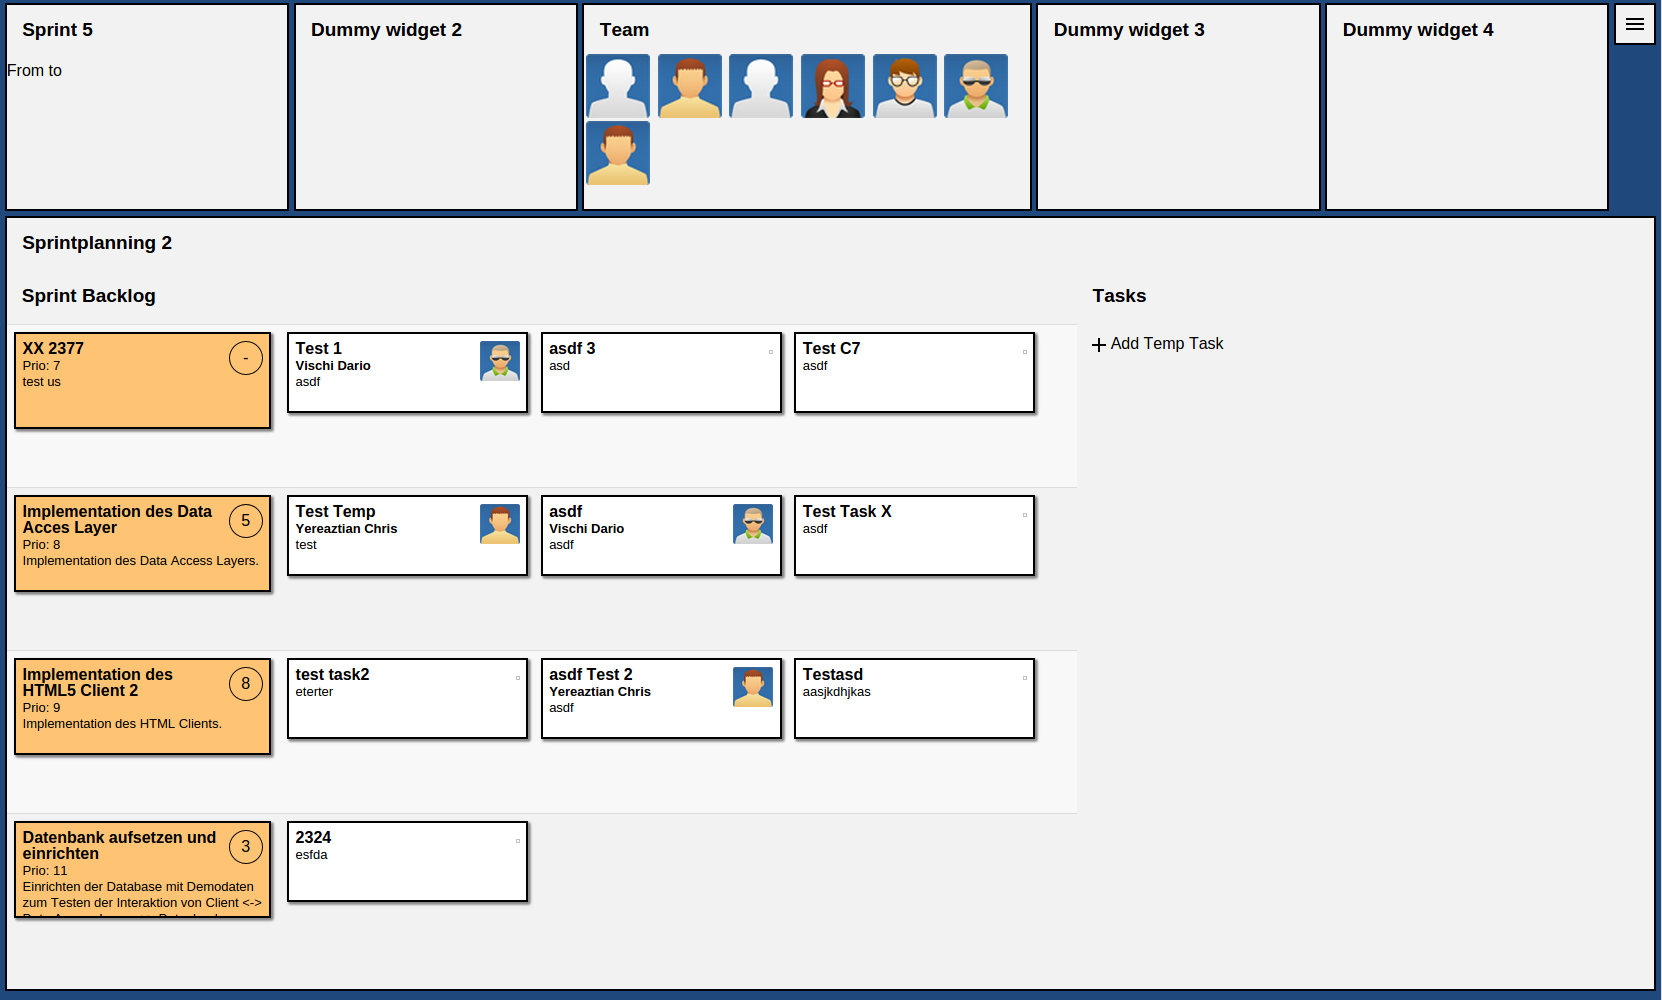
\includegraphics[width=\columnwidth]{figures/awall-layout}
	\caption{UI layout of Awall on a device larger than a tablet but smaller than the wall.}~\label{fig:awall-layout}
\end{figure}

% info view and widgets
The info-view is the horizontal panel at the top with the smaller widgets.
% responsiveness of number of widgets in the layout (min. width for widgets)
The widgets in the info-view can have different widths from standard width to multiple-times the standard-width.
The number of widgets to display is calculated by the application and depends on the width of the viewport.
This ensures that the widgets always have enough space.
The widgets that do not fit can be accessed by the workspace menu, where each widget can be enabled or disabled. 

% workspace menu
% workspace menu: save/reset workspace, list of widgets with toggle to en/disable, list of available meeting workspaces
The workspace menu is the small button in the top right corner.
It allows to control which widgets are enabled and disabled with toggles, to switch to other workspaces and to save or reset the current workspace configuration.

% main widget
The main widget is the largest part of the UI and is the main working area.
For the daily stand-up meeting, it displays the taskboard.
For each meeting of the agile process there is a specialized main widget that shows exactly what is needed and offers tailored interaction methods.
% responsiveness of sp2 workspace; 2 "layouts": large screen and small screen (sprint view: show all US, US view: show selected US and all tasks + temp tasks)
Each main widget is responsible for the responsive behavior if its content to show the appropriate amount of information depending on the available space.
Since we have a very large screen for the wall and a smaller screen for the tablets, we have two layouts for the \gls{sp2} main widget.
The layout for the large screen shows all the available information at once.
That specifically means all user stories including their already created and assigned tasks plus all tasks that were just created but have not been assigned to a user story yet.
For tablet-sized displays, the small-screen layout consists of two views.
The first view shows all user stories in a grid.
When the user clicks respectively selects a user story, the second view is shown.
In the detail view, the selected user story with all its tasks and the list of unassigned tasks is displayed.


% widget abilities (dock, resize etc)
The widgets in Figure~\ref{fig:awall-layout} are in a docked position but can be undocked by dragging them out of the info-view.
Once undocked, the widget can be moved around the viewport and resized by either using the mouse or the pinch-to-zoom gesture on a multi-touch display. 
% widgets sizes (title, default, full, edit mode)
The widgets can have different layouts for different sizes when being resized.
In the docked position in the info-view the widgets show the default layout on larger screens. 
% responsiveness of the layout (widget height with title only and default size)
On smaller screens like on a tablet, only the title of the widget is shown.
The default size with the same functionality as on larger screens is shown when it is undocked.
Besides the title-only and the default layout, a widget can offer an additional full layout and an edit mode.
The full layout is intended to show more information on the widget's subject or offer additional interaction functionality.
It is triggered by specifying the breakpoints for the width and height.
Once the widget has exceeded both breakpoints while resizing, the full layout is shown.
% - buttons when undocked (dock, reset size, enter edit mode)
If a widget has an edit mode, an edit icon is displayed in the top-right corner of the widget.
There are two more buttons on all widgets: one to reset the size to the default layout and one that docks the widget in the info-view.


% CHALLENGES

\begin{figure*}
	\centering
	\begin{subfigure}[b]{1\columnwidth}
		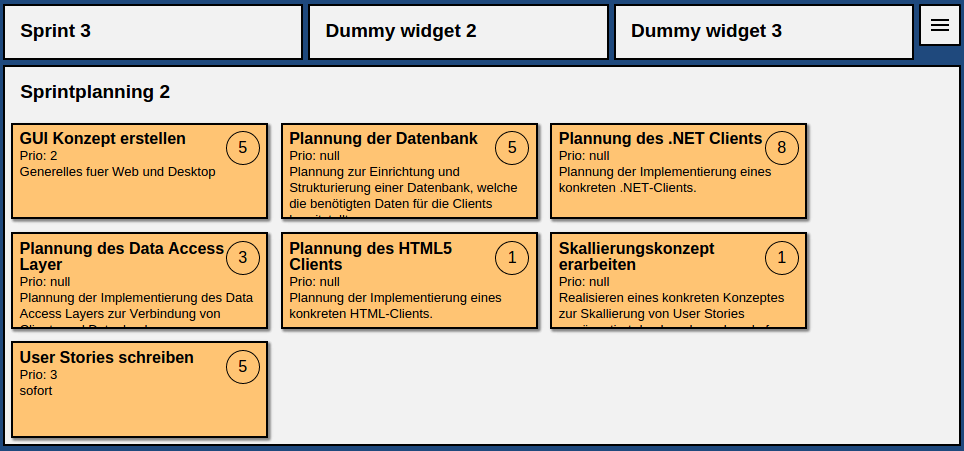
\includegraphics[width=\textwidth]{figures/sp2-overview}
		\caption{Overview}
		\label{fig:sp2-overview}
	\end{subfigure}%
	\quad
	\begin{subfigure}[b]{1\columnwidth}
		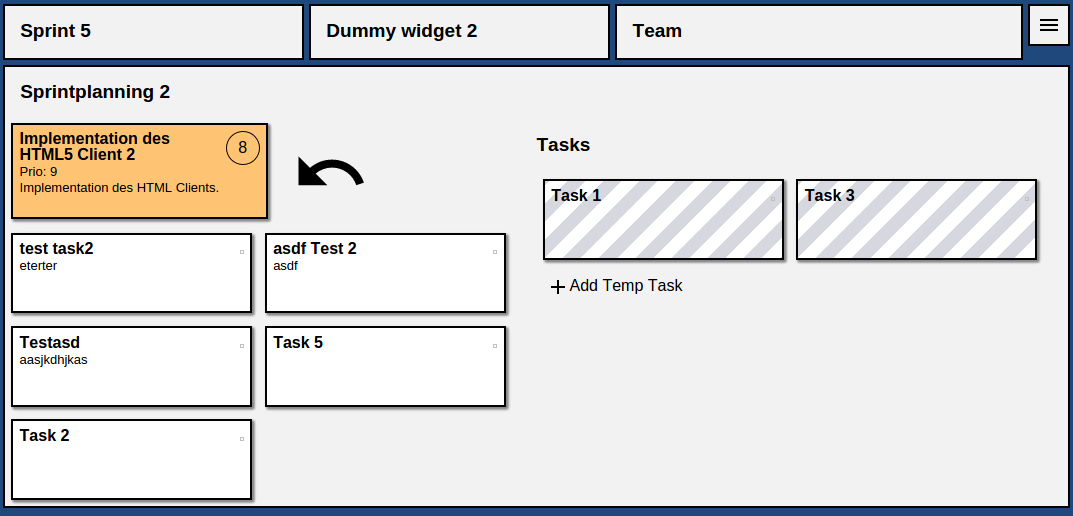
\includegraphics[width=\textwidth]{figures/sp2-detail}
		\caption{Detailed view}
		\label{fig:sp2-detail}
	\end{subfigure}
	
	\caption{The two views of the split up \gls{sp2} user interface for smaller displays.}\label{fig:animals}
\end{figure*}

% same functinality, smaller screen
Even though the screen of tablet is not as small as a smartphone, bringing an UI designed for a large wall to such a device presents some challenges.
An important aspect was to retain the same functionality on the tablet as on the wall.

% title-only view => undock => default view
A lot of vertical space is used up by the info-view widgets.
They offer auxiliary functionality, but it is not absolutely essential that they are completely visible the whole time in their default layout.
Thus, we created the title-only layout for the widgets.
That way the widgets are still in the same place and visible, but have to be undocked to use.
When the widget is undocked it enlarges to the default size and it can be used like on the wall.
% thinking more about the widgets => full and edit mode
By thinking about the widgets and how to use them, we also extended the functionality with the full layout and the edit mode.
% visibility of information (tablet: single person (focused), wall: many people(overview))
In our collaborative scenario of the \gls{sp2} meeting, the wall and the tablet serve different needs.
While the wall is used for overview in the collaborative discussion, the tablet is used by an individual to create the task for the currently discussed user story.
That means that the layout and the amount of information displayed in the main widget can differ.
% multiple layouts for a single widget (sp2 overview, detail view)
So for our scenario, the full list of user stories is not important for the individual while creating a task on the tablet.
Thus, we have split the widget into two views, an overview (Figure \ref{fig:sp2-overview}) and a detail view (Figure \ref{fig:sp2-detail}), as mentioned above.

\section{Architecture}

%- System overview (Server, JIRA, REST API)
The whole system consists of four components:
\begin{itemize}
	\item Awall web application: The Awall application is a \gls{spa} and is built using HTML, Javascript and CSS.
	\item A web server: A web server delivers the Awall web application files to clients.
	\item Application server: An application server that provides a REST API for Awall to retrieve the data about the sprints, user stories, tasks and team members.
	It also provides a WebSocket endpoint for real-time updates.
	\item A data backend: The data used by the REST API is provided by a backend. 
	Currently, the system uses a JIRA backend. JIRA is a bug, issue and project management software used by many software development teams around the world.
\end{itemize}

% Awall web app delivered by the web server:
Awall is a \gls{spa}, that means that the website is not rendered by an application server and then sent to the client but is rendered completely on the client.
It also means that the website does not reload, even when another page of the website is loaded. 
The resources like images and scripts are loaded dynamically when needed and added to the application at runtime.
The information about sprints, user stories and tasks is retrieved from the application server over the REST API.
The data is delivered in a light-weight format called JSON. 

%- HTML5 WebComponents to isolate functionality (JS) and style (CSS)
Awall uses Web Components \cite{webcomponents.org}, a set of four standards currently being produced as a W3C specification.
Those four specifications offer the following features that can be used together or individually:
\begin{itemize}
	\item Custom Elements: Define and use new HTML elements. 
	That ranges from simple format-elements to complex elements with functionality like for example the HTML5 video element.
	\item HTML Imports: Include and reuse HTML documents.
	Allows to define custom elements in a separate file,  import it and then use those custom elements. 
	Similar to how CSS and Javascript files can be imported.
	\item Templates: Declare inert \gls{dom}-trees that can be reused to instantiate custom elements.
	\item Shadow DOM: Encapsulate functionality and style in \gls{dom}-trees.
	CSS definitions are by default global no matter where they are defined.
	By encapsulating the style definitions in a Shadow DOM, they become local and do not affect any other \gls{dom} elements.
\end{itemize}

%- nested, reusable elements instead of MVC
The application is composed of nested custom HTML elements and does not follow the more traditional MVC pattern. 
This approach goes more in the direction of component-based software engineering that emphasizes the separation of concerns.
The custom elements can be defined in separate HTML documents and be reused in multiple web applications by importing the document.
This also means that the elements can be loosely-coupled and independent.
Even the access to the REST API is encapsulated in an element. 
To use the REST API, another element only needs to instantiate the appropriate custom element by inserting the corresponding HTML tags into its own HTML.



%- Workspace config/definition in a json file (widget position, width, hidden)
The workspaces that make up the web application are configured in JSON files. 
Apart from a name and the description for the workspace, a path, a layout and widgets must be defined. 
% path property
The path is the fragment identifier '\#' of the URL including variables that are required by the given workspace.
For example "/project/:projectId/sprint/:sprintId/sp2" is the path for the \gls{sp2} worksapce.
':projectId' and ':sprintId' are the variables required for that workspace and the complete URL for this workspace is "http://example.com/\#/project/ATBD/sprint/10204/sp2".
% layout property
A workspace must define which layout to use.
It defines how the widgets are arranged and how many widgets besides the main widget are shown.
It also defines whether additional visual elements like the workspace menu are visible.
Currently there are two layouts, more can be added if desired.
One is for simple selection pages like selecting the sprint that only has a main widget.
The other is the workspace layout as seen in Figure~\ref{fig:awall-layout} with the widgets panel at the top and the main widget.
% widgets property
The widgets property defines which widgets occupy which position in the layout.
Each layout must at least have a main widget.
The others are configured with a positional attribute that defines the order in the top panel, a visibility attribute and a width attribute.

% how the application is loaded (simple)
The web application loads all workspace configuration files first, then determines which workspace to load by examining fragment identifier of the URL.
The requested workspace is then loaded by importing the HTML file that defines the layout and all the defined widget's HTML files.
Some custom elements are used in multiple widgets and are thus defined in their own HTML document.
For example the custom element that represents a task, called taskcard, is defined in taskcard.html and imported by the widgets that use it.
Those elements are imported directly by using the HTML Imports specification.
Once the layout and the widgets have been loaded, the widgets are instantiated and inserted into the layout according to their configuration attributes like position and width.
The layout is then set as the body of the HTML \gls{dom}-tree.

%-How information is propagated (e.g. new task created)
%-> WebSocket message to all clients (replace in-place, no website reload)
The REST API alone only offers communication by means of request and response.
To make the application more dynamic, the application server also offers a WebSocket \cite{websocketRFC} endpoint.
WebSocket is full-duplex communication protocol designed to be implemented by web browsers and web servers.
It allows both participants (client and server) to send asynchronous messages for real-time communication.
Once the client has established the connection, it is persistent until closed explicitly.
WebSocket allows the web application not only to recognize changes made by itself, but also changes made by other instances of the web application on different devices no matter where they are.
This works because all instances of the web application establish a WebSocket connection to the application server when started.
If, for example a task has been modified, the task is saved by the application server in the backend and then the information is propagated to all clients over the WebSocket connection.
When the web application receives an update, it checks whether the current workspace uses this task.
If that is the case, the task is updated in-place without reloading the page.
Has a task been created for a user story, it will pop-up on all connected devices in real-time.

% cornerstones of rwd
For the UI, the web application uses an approach called \gls{rwd} that builds on three cornerstones:
\begin{itemize}
	\item Relative units: The style and layout definitions should use relative units like percent instead of fixed units like pixel. A pixel is on a 1080p smartphone display is not the same size as a pixel on a 1080p 24" desktop display. 
	\item Flexible images: The images are sized in relative units but there may also be multiple versions of the same image. For example a low resolution image for small-screen devices and a higher resolution image for larger devices.
	\item Media Queries: Media Queries are the main cornerstone of \gls{rwd}. They allow us to define breakpoints with conditional statements in the stylesheet at which different CSS style definitions take effect.
\end{itemize}

Media Queries have been introduced in CSS3 and became a W3C standard in June 2012 \cite{mediaqueriesW3C}.
They allow the content of a website to adapt to the conditions of the web browser.
The most prominent example of such a condition is the screen resolution.
By defining break-points, using for example the width of the viewport, the statement defines the style of the given \gls{dom} element.
% media query example
Let's assume we have a simple element with a title in h1-element and a text in a p-element.
The Media Query could define that the p-element is hidden when the height of the viewport is less than 500 pixels.


\section{Implementation}
%- Polymer, Interact.js
The implemented Awall web application uses the Polymer~\cite{polymer}, a library that abstracts WebComponents and allows to define custom elements using declarative HTML tags instead of pure Javascript code.
This makes it easy to write new custom elements without a huge amount of boilerplate code that is required when using the native Javascript APIs directly.
For multi-touch gestures like pinch-to-zoom, drag\&drop and resizability of elements, Awall uses the interact.js~\cite{interactJs} library.

%WIDGETS
%- support drag&drop and resize with mouse and pinch-to-zoom
%- multiple layouts for widgets (sizes)
%-- <awall-widget>, <awall-widget-size-default> etc.
The different layouts of the widgets are implemented using custom elements.
All widgets must place their content in the custom element tag \textless{}awall-widget\textgreater.
This gives them features like resizability and drag\&drop.
For the title-only mode to work, the widget must use the element \textless{}awall-widget-title\textgreater to define its title.
The default content is also contained in the element\textless{}awall-widget-size-default\textgreater.
To fully utilize the resize functionality and support the full layout of a widget, the content for this layout must be placed in the element \textless{}awall-widget-size-full\textgreater.
The edit mode also has its own element: \textless{}awall-widget-editable\textgreater.
 
All elements except title-only are enclosed in an element whose visibility is controlled by a Media Query.
As long as the browsers viewport height is smaller than a defined breakpoint, only the title of the widget is shown and the height of the widget is only as high as the title.
During resizing, the width and height of the widget are compared to the breakpoints.
Once both breakpoints have been exceeded, the default layout is is hidden and the full layout is displayed.
The edit mode is controlled by the user by means of a button in the widget.


\section{Discussion and Future Work}

% discussion Awall (how great it is)
The framework we developed with Awall show, that current web technologies and emerging new web standards make it possible to build a responsive web application for different sized devices. 
The fact that it is an \gls{spa} and uses asynchronous messages for updates over WebSockets allows the application to run on multiple devices with the displayed data always up-to-date without the need to reload the website.
The framework is also designed to be easily extendable with additional workspaces, layouts and widgets.
Through its design using loosely-coupled components or in the web context custom elements, there are no dependencies between the widgets.

%results from taskboard UI tests (-> tasks for future work)?
After the design of the large-screen UI, we conducted some live-action interviews with developers to discover if the wall could be something they want to work with and to get input on how to improve it.
%meetings with a distributed team (e.g. show movement when a task is dragged) [similar to PolyChrome]
In the future, we are going to build on the input we received and would also like to extend the wall to work with distributed teams, where the movements  of a task for instance are mirrored on other walls.
%handwriting ability


\balance{}

% REFERENCES FORMAT
% References must be the same font size as other body text.
\bibliographystyle{SIGCHI-Reference-Format}
\bibliography{references}

\end{document}

%%% Local Variables:
%%% mode: latex
%%% TeX-master: t
%%% End: